\documentclass[oneside, a4paper, 12pt, chapter=TITLE]{abntex2} 	% fleqn - alinha equações à esquerda
\usepackage{UFBA}												% Edição de alguns quesitos no estilo do manual da UFBA
\usepackage[T1]{fontenc}										% Seleção de códigos de fonte.
\usepackage[utf8]{inputenc}										% Codificação do documento (conversão automática dos acentos)
\usepackage{lmodern}											% Usa a fonte Latin Modern
																% Para utilizar a fonte Times New Roman, inclua uma % no início do comando acima  
																% Abaixo, tire a % antes do comando  \usepackage{times}
%\usepackage{times}		    									% Usa a fonte Times New Roman				
\usepackage{lastpage}											% Usado pela Ficha catalográfica
\usepackage{indentfirst}										% Indenta o primeiro parágrafo de cada seção.
\usepackage{color}												% Controle das cores
\usepackage{graphicx}											% Inclusão de gráficos
\usepackage{float} 												% Fixa tabelas e figuras no local exato
\usepackage{subfig}												% para inserir mais figuras
\usepackage{microtype} 											% para melhorias de justificação
\usepackage{makeidx}           									% para gerar índice remissimo
\usepackage{hyperref}											% para configurações do pdf
\usepackage{amsmath}											% para alguns formatos de equações
\usepackage{amssymb}											% para mais símbolos
\usepackage[portuguese,			
			linesnumbered, 										% linhas numeradas
			commentsnumbered,									% comentários numerados
			boxed												% com caixa ao redor
			]{algorithm2e}  									% para escrever os algoritmos
\usepackage{listings}											% para colocar códigos de programas		
\usepackage{scrextend}
\usepackage{pdfpages}											% Para incluir páginas em pdf
\usepackage{multicol}											% Suporte a mesclagens em colunas
\usepackage{multirow}											% Suporte a mesclagens em linhas
\usepackage{longtable}											% Tabelas com várias páginas
\usepackage{threeparttablex}    								% notas no longtable
\usepackage{array}
\usepackage[alf,abnt-emphasize=bf, abnt-thesis-year=both, abnt-repeated-author-omit=yes, abnt-last-names=abnt, abnt-etal-cite,abnt-etal-list=3, abnt-etal-text=default, abnt-and-type=e, abnt-doi=doi, abnt-url-package=none, abnt-verbatim-entry=no,bibjustif]{abntex2cite}


\renewcommand{\footnotesize}{\small}
\autor{Nome do autor} 
\titulo{Título do trabalho} 
\data{2021} 
\local{Salvador} 
\preambulo{Trabalho de conclusão de curso de ***, como pré-requisito para obtenção do grau de Bacharel em ***, pela \imprimirfaculdade{} da \imprimirinstituicao. } 
\instituicao {Universidade Federal da Bahia}
\faculdade {Ex: Escola Politécnica}
\programa {Ex: Departamento de Construção e Estruturas}
\orientador{Ex: Prof. Dr. Não Orienta em Nada e Cobra} 
\tipotrabalho{Ex: Trabalho de Conclusão de Curso}
% ---
% ---
% compila o sumário e índice
\makeindex
% ---
% ---
% ----------------------------------------------------------
% INFORMAÇÕES DO PDF
% ----------------------------------------------------------
% alterando o aspecto da cor azul e vermelho
\definecolor{blue}{RGB}{25,25,112}
\definecolor{red}{RGB}{128,0,0}
\makeatletter
\hypersetup{
	%pagebackref=true,
	pdftitle={\@title}, 
	pdfauthor={\@author},
	pdfsubject={\imprimirpreambulo},
	pdfcreator={LaTeX with abnTeX2},
	pdfkeywords={abnt}{latex}{abntex}{UFBA}{trabalho acadêmico}, 
	colorlinks=true,       	    % false: boxed links; true: colored links
	linkcolor=blue,          	% color of internal links
	citecolor=red,        		% color of links to bibliography
	filecolor=magenta,      	% color of file links
	urlcolor=black,
	bookmarksdepth=4
}
\makeatother
% --- 
% Espaçamentos entre linhas e parágrafos 
% --- 
% Simbolo -1 inverso
\newcommand{\inv}{^{\raisebox{.2ex}{$\scriptscriptstyle-1$}}}
% O tamanho do parágrafo é dado por:
%\setlength{\parindent}{1.0 cm}
\OnehalfSpacing

% Controle do espaçamento entre um parágrafo e outro:
\setlength{\parskip}{6pt} 
% ---
% ---
% Renomear Figuras, Algoritmos e Equações no autoref
% ---
\renewcommand{\algorithmautorefname}{Algoritmo}
\renewcommand{\equationautorefname}{Equação}
\renewcommand{\figureautorefname}{Figura}
\renewcommand{\tableautorefname}{Tabela}
\renewcommand{\chapterautorefname}{Capítulo}
\newcommand{\subfigureautorefname}{\figureautorefname}

\renewcommand{\sfdefault}{\rmdefault} %Para definir a fonte latex como padrão definida em escopo o documento

% ---
% ---
% ----------------------------------------------------------
% INÍCIO DO DOCUMENTO
% ----------------------------------------------------------
\begin{document}

% Seleciona o idioma do documento (conforme pacotes do babel)
\selectlanguage{brazil}
% Se o idioma do texto for inglês, inclua uma % antes do 
%      comando \selectlanguage{brazil} e 
%      retire a % antes do comando abaixo
%\selectlanguage{english}

% Retira espaço extra obsoleto entre as frases.
\frenchspacing 

% --- Formatação dos Títulos
\renewcommand{\ABNTEXchapterfontsize}{\fontsize{12}{12}\bfseries}
\renewcommand{\ABNTEXsectionfontsize}{\fontsize{12}{12}}
\renewcommand{\ABNTEXsubsectionfontsize}{\fontsize{12}{12}\normalfont\bfseries}
\renewcommand{\ABNTEXsubsubsectionfontsize}{\fontsize{12}{12}\normalfont}
\renewcommand{\ABNTEXsubsubsubsectionfontsize}{\fontsize{12}{12}\normalfont}

% --- Formatação da fonte do Sumário
\renewcommand{\cftsectionfont}{\normalsize}
\renewcommand{\cftsectionpagefont}{\cftsectionfont}
% 
\renewcommand{\cftsubsectionfont}{\bfseries}
\renewcommand{\cftsubsectionpagefont}{\cftsubsectionfont}
% ----------------------------------------------------------
% ELEMENTOS PRÉ-TEXTUAIS
% ----------------------------------------------------------
% ---
% Capa
% ---
\imprimircapa
% ---
%Folha de Rosto
% ---
\imprimirfolhaderosto
% ---
% Folha de aprovação
% --- NÂO RETIRAR ESPAÇO ABAIXO

\begin{folhadeaprovacao}
\begin{center}
	\textbf{\MakeUppercase{\ABNTEXchapterfont\large\imprimirautor}}
\end{center}

\begin{center}
	  \textbf{\MakeUppercase{\ABNTEXchapterfont\Large\imprimirtitulo}}
\end{center}
%\MakeUppercase{\ABNTEXchapterfont\bfseries\large\imprimirsubtitulo}
%\vspace{1cm} 
\vspace*{\fill}

\begin{flushleft}
	\imprimirpreambulo
\end{flushleft}
\vspace*{\fill}

Trabalho aprovado. \imprimirlocal, xx de mês de \imprimirdata.

\begin{center}
	\bfseries{Banca Examinadora}
\end{center}
\assinatura{\textbf{\imprimirorientador} \\ Orientador -- UFBA} 
\assinatura{Prof. Dr. Professor 01 \\ Convidado -- UFBA}
\assinatura{Eng. Engenheiro convidado 01 \\ Convidado -- UFBA} 
\assinatura{Eng. Engenheiro convidado 02 \\ Convidado -- UFBA}
\vfill
\OnehalfSpacing
\begin{center}
	{\large\imprimirlocal}
	\par	
	{\large\imprimirdata}
\end{center}
\end{folhadeaprovacao}
% ---
%Ficha catalográfica. gerar ficha no site: https://sibi.ufba.br/modelo-de-ficha-catalografica-geracao-automatica
% ---
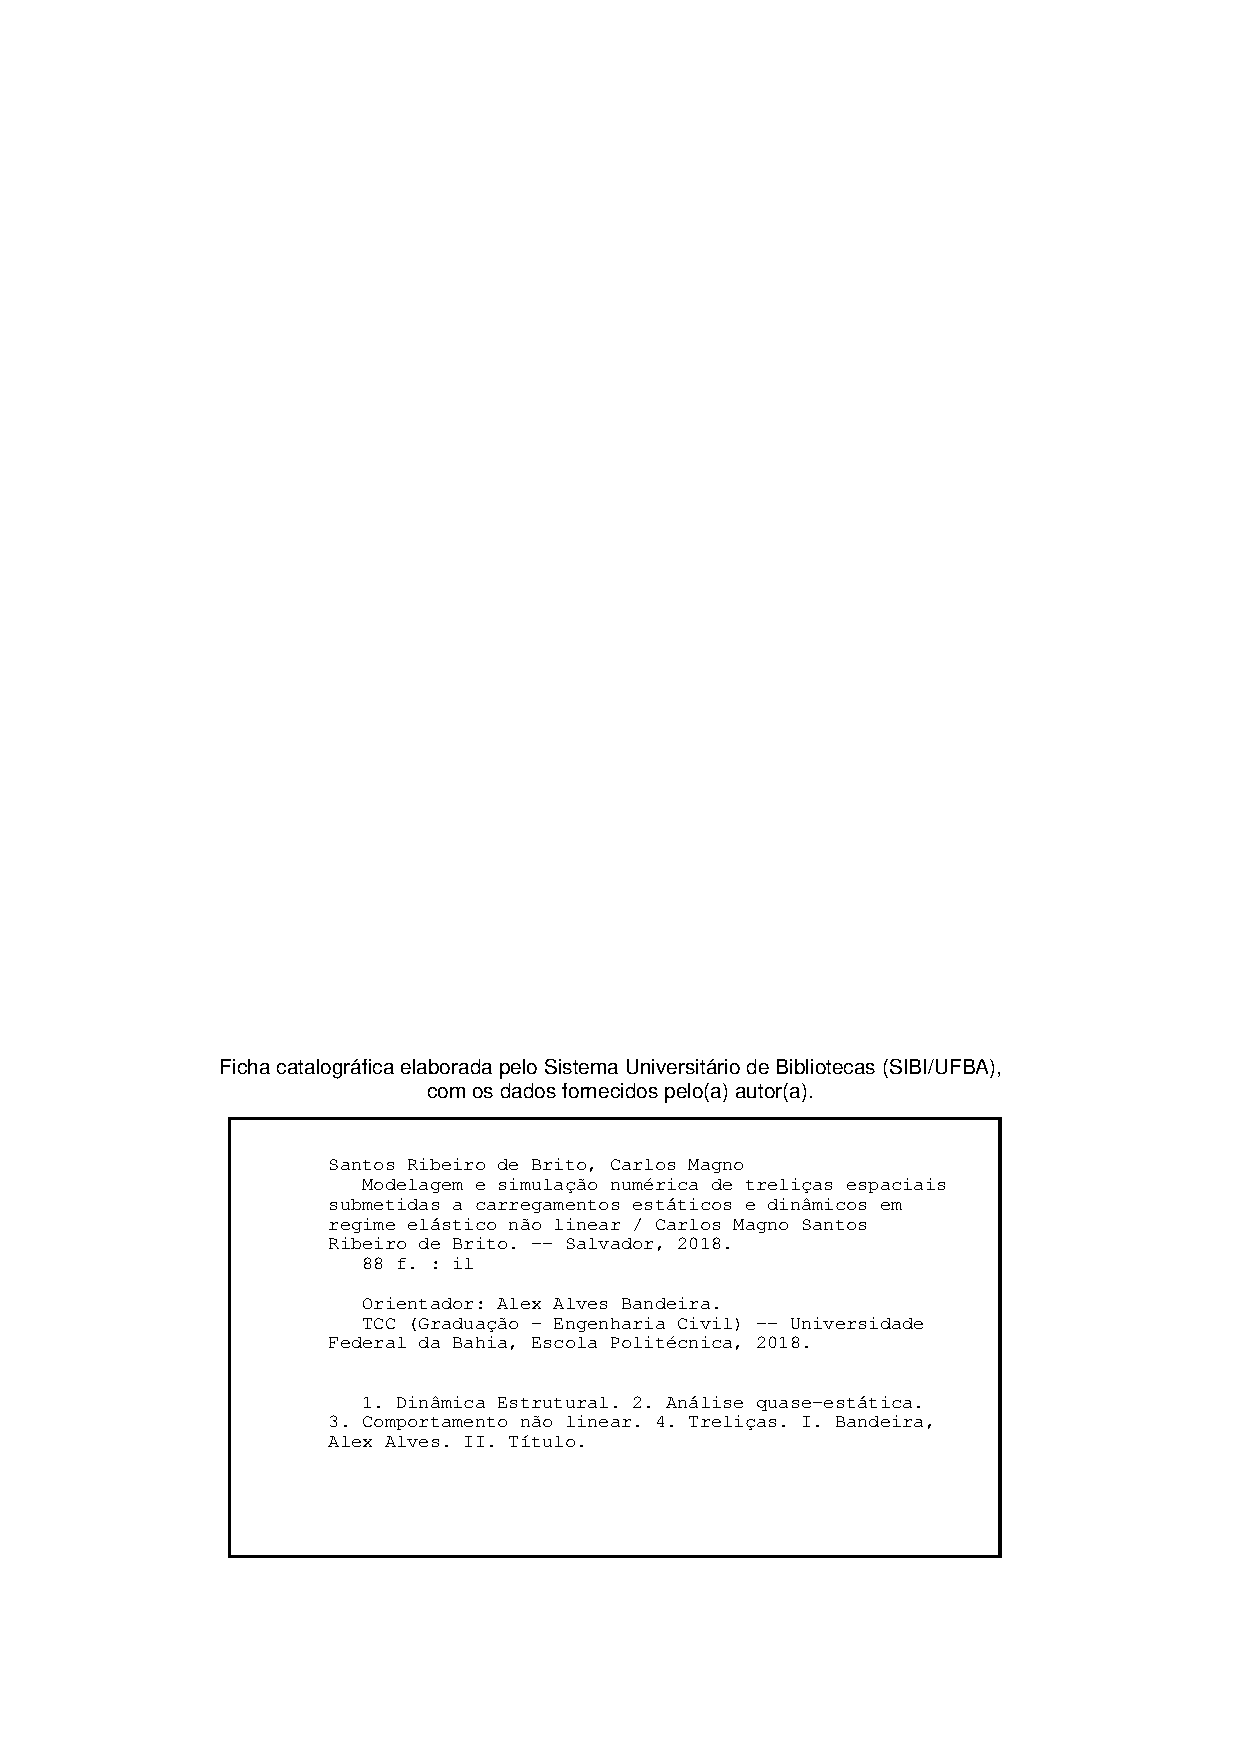
\includepdf{ficha.pdf}
% ---
% Dedicatória e agradeciemento
% ---
%dedicatória e agradecimentos
% ---
% ---
\begin{dedicatoria}

	\vspace*{\fill}
	À ...
	\vspace*{5cm}
\end{dedicatoria}
% ---
\begin{agradecimentos}
	
	Dedico à...
	
\end{agradecimentos}
% ---
% ---
% Epígrafe
% ---
\begin{epigrafe}
	\vspace*{\fill}
	\begin{flushright}
		Inserir aqui epígrafe caso queira\\
		\vspace*{1cm}
		Nome do Autor (Ano, p.39)
	\end{flushright}
\end{epigrafe}
% ---
% Resumo (Português)
% ---
%% Resumo.tex
% ---
% Resumo
% ---
	\setlength{\parindent}{0pt}
	\setlength{\absparsep}{0pt} % ajusta o espaçamento da referência	
	\SingleSpacing 
	BRITO, C. M. S. R. \imprimirtitulo. \pageref{LastPage} f. \imprimirdata. \imprimirtipotrabalho~-~\imprimirfaculdade, \imprimirinstituicao, \imprimirlocal, \imprimirdata. 
	%Substitua p. por f. quando utilizar oneside em \documentclass
	%\pageref{LastPage}f.
\vspace{ 0.5 cm} 	
\begin{resumo}
\SingleSpacing
Resumo do trabalho
\\
\\
\textbf{Palavras-chave}: Palavra1, Palavra2, Palavra3, Palavra4. % Até 5 palavras 
\end{resumo}

% ---
% Resumo (inglês e outras línguas a desejar)
% ---
%\begin{resumo}[Abstract] 
%\begin{otherlanguage*}{english}		
%\end{otherlanguage*}
%\end{resumo}
% ---
% inserir lista de figuras
% ---
\pdfbookmark[0]{\listfigurename}{lof}
\listoffigures*
\cleardoublepage
% ---
% ---
% inserir lista de tabelas
% ---
\pdfbookmark[0]{\listtablename}{lot}
\listoftables*
\cleardoublepage
% ---
% ---
% inserir lista de Algoritmos
% ---
\pdfbookmark[0]{Lista de algoritmos}{loa}
\listofalgorithms
\cleardoublepage
% ---
% ---
% inserir lista de abreviaturas e siglas (Caso Haja)
% ---
%\begin{siglas}
%	\item[ABNT] Associação Brasileira de Normas Técnicas
%	\item[abnTeX] Normas para TeX
%\end{siglas}
% ---
% ---
% inserir lista de símbolos
% ---
%Pode-se alterar para uma forma automática de simbologia. Exemplos(não auromáticos):
\begin{simbolos}
	\item[$\boldsymbol f_i$, $f_i$]\quad Vetor das forças internas, força interna
	\item[$\boldsymbol f_e$, $f_e$]\quad Vetor das forças externas, força externa
	\item[$\boldsymbol u$, $u$]\quad Vetor dos deslocamentos nodais, deslocamento nodal
	\item [$\varepsilon$]\quad Deformação longitudinal
	\item [$L_i$]\quad Comprimento referência, inicial
	\item [$L_f$]\quad Comprimento atual
	\item [$\lambda$]\quad Alongamento linear ou estiramento
	\item[$\boldsymbol f_e(t)$]\quad Vetor das forças externas variantes no tempo
	\item[$\omega$]\quad Frequência
	\item[$\omega_{n}$]\quad Frequência natural
	\item [$\boldsymbol K $, $ k $]\quad Matriz de rigidez, rigidez
\end{simbolos}
% ---
% ---
% inserir lista de siglas
% ---
%Pode-se alterar para uma forma automática de simbologia. Exemplos (não automáticos):
\begin{siglas}
	\item[MEF]\quad Método dos elementos finitos
	\item[PTV]\quad Princípio dos trabalhos virtuais
	\item [Ansys]\quad Swanson Analysis Systems, Inc.
	\item[DTruss]\quad Programa desenvolvido
\end{siglas}
% ---
% ---
% inserir o sumario
% ---
\pdfbookmark[0]{\contentsname}{toc}
\tableofcontents*
\cleardoublepage
% ---
% ---
% Numeração nas páginas:
\textual
% ---
% ---
% Espaçamentos definidos para o texto
% ---
%\setlength{\absparsep}{1.5cm} % ajusta o espaçamento do texto seguinte	
\OnehalfSpacing
\setlength{\parindent}{1.0cm} % espaçamento dos parágrafos	
% ----------------------------------------------------------
% INTRODUÇÃO, DESENVOLVIMENTO E CONCLUSÕES
% ----------------------------------------------------------
\chapter{Introdução}

Não é obrigatório seguir o padrão de introdução aqui adotado, com seções referentes aos Objetivos, justificativa e Organização do trabalho.

\section{OBJETIVOS}

\section{JUSTIFICATIVA}

\section{ORGANIZAÇÃO DO TRABALHO}


% ---
\chapter{Fundamentação Teórica}


\section{CARACTERÍSTICAS DA LINEARIDADE} \label{Sec:caraclinearidade}


\section{A NÃO LINEARIDADE} \label{Sec:anaolinearidade}


\subsection{Não Linearidade Física}


\subsection{Não Linearidade Geométrica} 


\section{DESLOCAMENTO E DEFORMAÇÃO} \label{Sec:deslocedeform}

\subsection {Deformação de Engenharia} \label{Sec:desloceng}

\section{CAMINHOS DE EQUILÍBRIO} \label{Sec:caminhodeequilíbrio}


\section{DINÂMICA ESTRUTURAL} \label{Sec:dinamicaestrutural}
 

\subsection{Ações dinâmicas}

\subsection{Sistema estrutural dinâmico}

\subsection{Expansão para vários graus de liberdade} \label{Sec:Expans}

\subsection{Sistema não amortecido e introdução à análise modal} \label{Sec:anlmodal}

\section{O AMORTECIMENTO}

% ---
\chapter{Métodos numéricos para análise estrutural}


\section{MÉTODO DE NEWTON-RAPHSON} \label{Sec:Metodonewtonraphson}

\section{MÉTODO DE NEWTON GENERALIZADO} \label{Sec:Metodonewtongeneral}

\section{MÉTODO DE NEWMARK} \label{Sec:Metodonewmark}


% ---
\chapter{Formulações matemáticas}\label{Sec:formulacoesmatematicas}
\section{MATRIZ DE RIGIDEZ TANGENTE} \label{Sec:matrizrigideztangente}

\section{PRINCÍPIO DOS TRABALHOS VIRTUAIS}\label{Sec:PTV}

% ---
\chapter{Implementação Computacional}


\section{VIGA TRELIÇADA}

\subsection{Análise dinâmica}

\section{DOMO TRELIÇADO}

\subsection{Análise estática}

\subsection{Análise dinâmica}

% ---
\chapter{Conclusão}

Digite aqui suas conclusões

%\section{SUGESTÕES DE TRABALHOS FUTUROS}

%Muitas possibilidades de ampliação do tema podem ser sugeridas com a finalização deste trabalho. Pode-se citar algumas:
%\begin{itemize}
%	\item 
%
%\end{itemize} 
%\input{Código}
% ----------------------------------------------------------
% ELEMENTOS PÓS-TEXTUAIS
% ----------------------------------------------------------
% -----------------------------------------------------------
% Referências bibliográficas
% ----------------------------------------------------------
% Exemplo de Referências sem citá-las no texto
\nocite{GID2017}
\nocite{Bandeira2001}
\nocite{Dominicio1977}
\nocite{Abrate1983}
\nocite{Martinelli2017}
% ----------------------------------------------------------
% ARQUIVO DE FONTE BIBLIOGRÁFICA (VER O JABREF OU MENDELEY)
% ----------------------------------------------------------
\bibliography{TCC_refs}

\end{document}
